
The TJ-Monopix1 chip series, as the name suggests, is fabricated by ToweJazz with 180 CMOS imaging process. Starting from the middle of 2010 (inteso come decina) a program with the goal to find a sensor suitable for future upgrade of experiments; the timeline in fig. \ref{fig:TJ180nm} shows the intermediate steps between the firt demonstrator and the successor of TJ-Monopix-1, TJ-Monopix2.\\
Not only TowerJazz, but also LFoundry with the same intention fabricated an other similar sensor with 150 CMOSS thecnology: both chip implemented a column drain read out with ToT cabability but while the LF-Monopix is a large-fill factor DMPAS, the TJ-Monopix has a small fill-factor electrode. DI QUALCOSA SU LF MONOPIX1
\begin{figure}[h!]
    \centering
    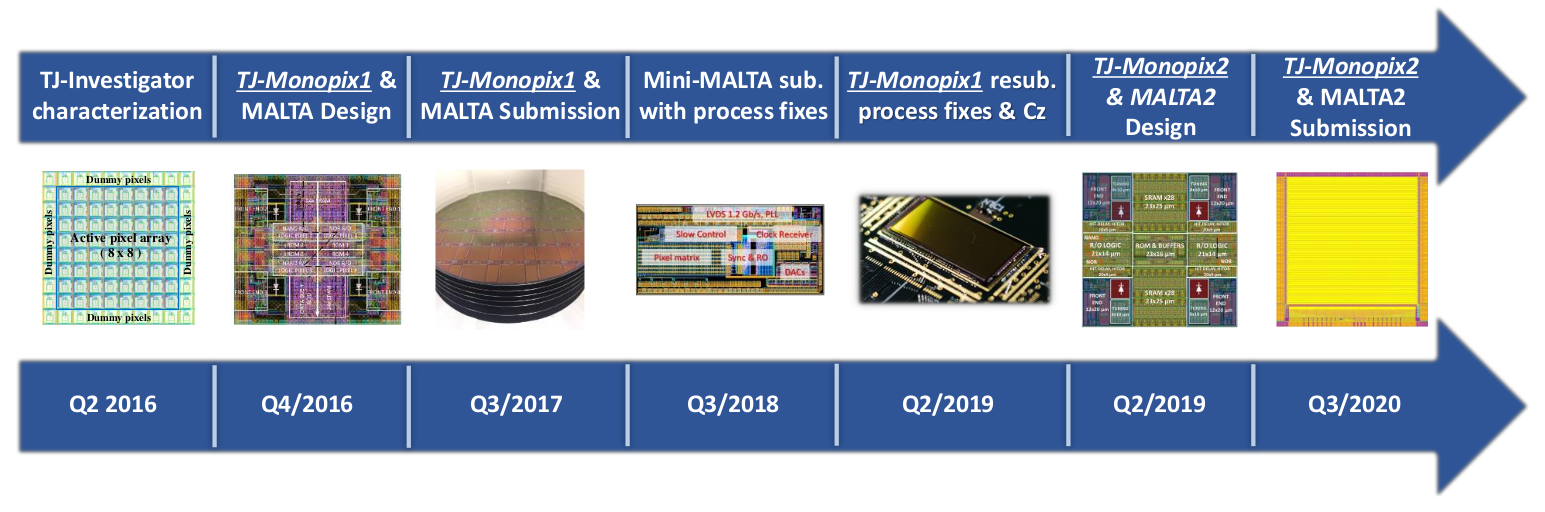
\includegraphics[width=.9\linewidth]{figures/Monopix1/TJ180nm.png}
    \caption{}
    \label{fig:TJ180nm}
\end{figure} 

\begin{table}
    \begin{center}
    \begin{tabular}{|c | c |c |}
    \hline
    & LF-Monopix & TJ-Monopix\\
    \hline
    \hline

    \hline
    \end{tabular}
    \caption{}
    \label{tab:LF-TJ-Monopix}
    \end{center}
 \end{table}

As already mentioned in chapter \ref{chap:}, in the timeline of Belle-II experiment should be include also the planning and the submission on Obelix, the heir of TJ-Monopix2. \\
DI QUALCOSA DI OBELIX.\\


\subsection{The sensor}
    \begin{table}
        \begin{center}
        \begin{tabular}{| c |c |}
        \hline
        Parameter & Value\\
        \hline
        \hline
        Matrix size & \\
        Pixel size & \\
        BCID & 40 MHz \\
        ToT-bit & 6 \\
        Power consumption & \\
        \hline
        \end{tabular}
        \caption{}
        \label{tab:LF-TJ-Monopix}
        \end{center}
    \end{table}
    TJ-Monopix adopted the modification I've told about in \ref{chap:} that allows to achive a full depletion: a planar low dose n implant is build on a high resistivity ($\geq $ 1 k$\Omega$ cm), p-type epitaxial layer.\\
    The modification improves a lot the performances of the detector, especially after radiation, but  Technology Computer Aided Design (TCAD) simulations(fig.\ref{fig:Monopix1_section_scheme}) have shown that a non uniform electric field is still produced in the substrate after the modification; since the lateral component of the electric field drops at the pixel corner (this point in figure is indicated by a star) the efficiency at the side is reduced. \\
    In some cases a second modification have been made then to increase the lateral component of electric field: a portion of low dose implant has been removed creating a discontinuity in the pixel corner. Questo migliora le prestazioni del rivelatore, ma dall'altra parte non rende più possibile fornire tensione separatamente a deep p well e substrate, sennò si ha punchthrought.\\

    \begin{figure}[h!]
        \centering
        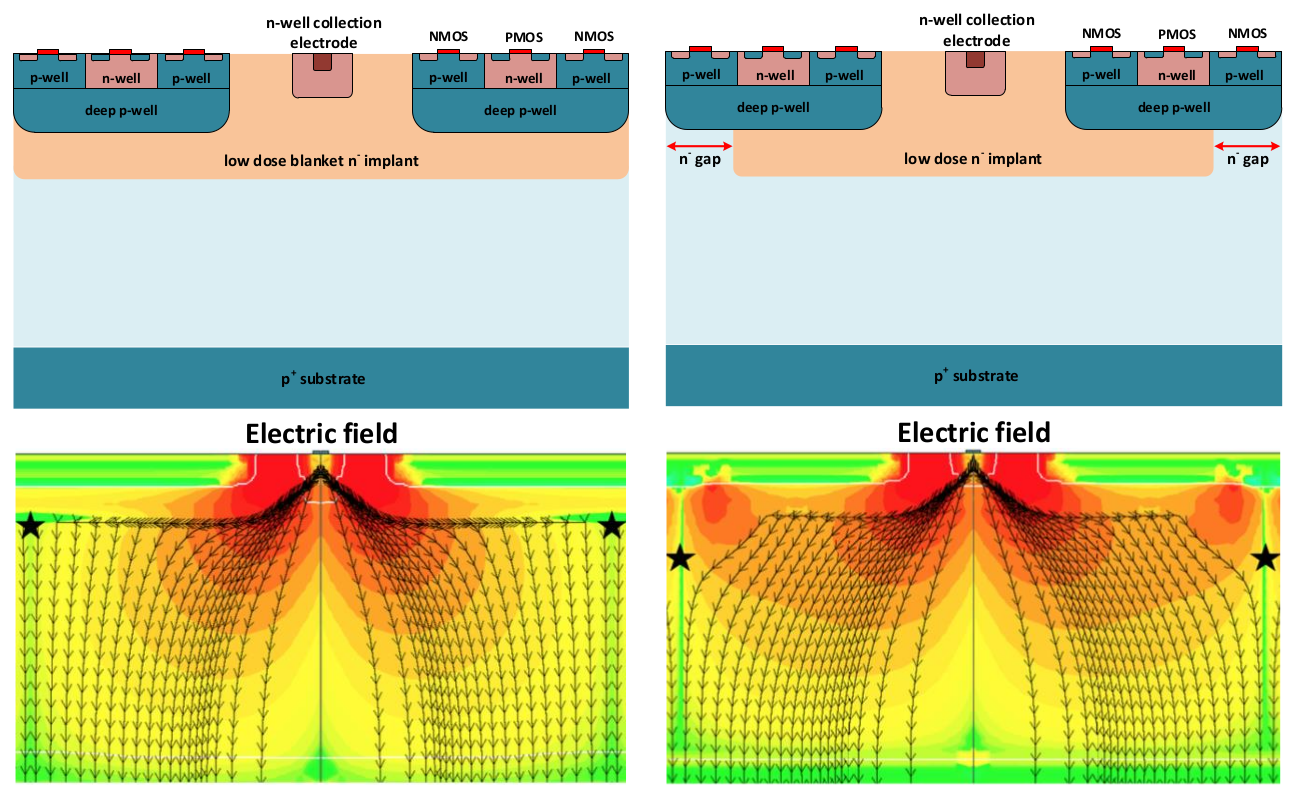
\includegraphics[width=.9\linewidth]{figures/Monopix1/Monopix1_section_scheme.png}
        \caption{(a) The cross-section of a monolithic pixel in the TJ-Monopix 180 nm with modified process; additionaly in (b) a gap in the low dose implant is created to improve the collection of charge due to a bigger lateral component of the electric field}
        \label{fig:Monopix1_section_scheme}
    \end{figure}

    C'è anche una differenza: portion e e non portion tra parte alta e bassa della matrice.\\


\section{FE flavors}
    TJ-Monopix1 has four different FE
    \begin{figure}[h!]
        \centering
        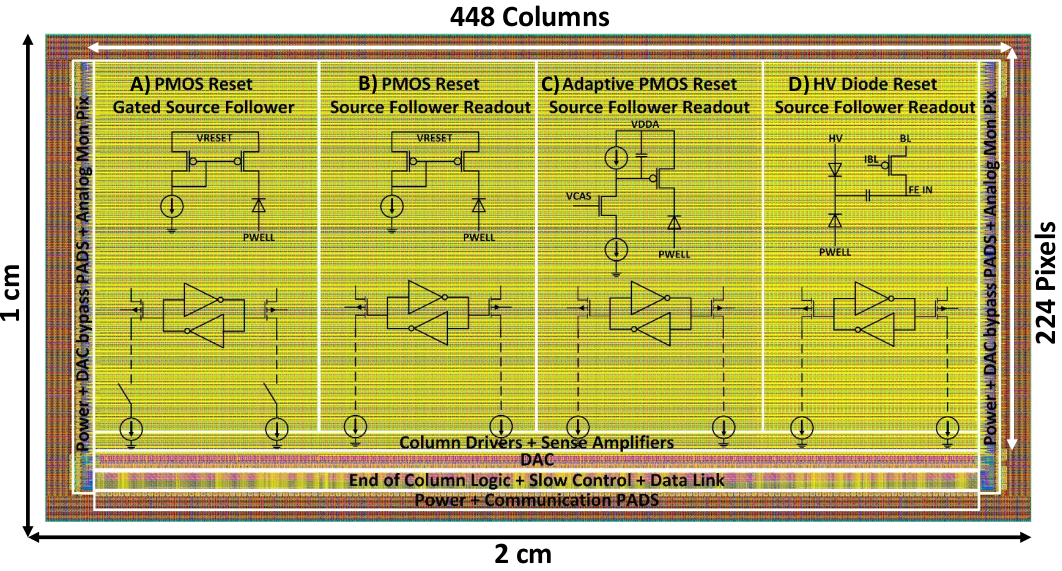
\includegraphics[width=.5\linewidth]{figures/Monopix1/Monopix1_flavors.png}
        \caption{}
        \label{fig:Monopix1_flavors}
    \end{figure}

    The FE circuit \ref{fig:Monopix1_FE_circuit} is ALPIDE-like, so it is similar to the one described in \ref{chap:}; a quanto già detto voglio però aggiungere due parole: come viene implementato il mascheramento dei pixels e il reset.\\ 
    Prevedere un modo di mascherare gli screaming pixel, tipicamente pixels con manufacturing defects, è fondamentale per poter ridurre il rate molto alto di dati e non saturare la banda. 
    \begin{figure}[h!]
        \centering
        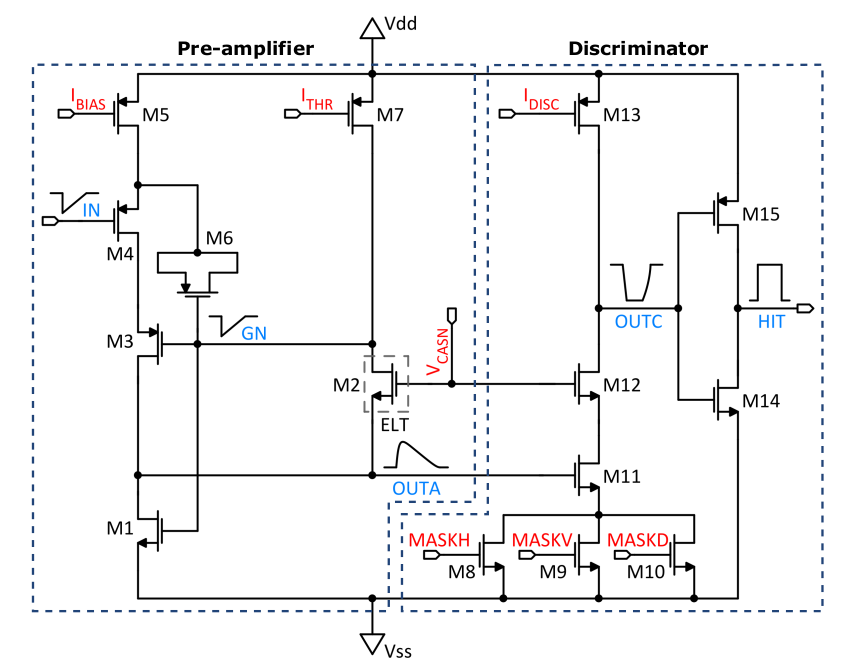
\includegraphics[width=.6\linewidth]{figures/Monopix1/Monopix1_FE_circuit.png}
        \caption{}
        \label{fig:Monopix1_FE_circuit}
    \end{figure}

    In the circuit in fig. \ref{fig:Monopix1_FE_circuit} transistors M8, M9 and M10 implement are used to disable pixels-readout, where MASKH, MASKV and MASKD represent respectivelly the vertical, orizontal and diagonal coordinates of the pixel that one want to mask. \\ 
    If all three transistors-signals are low, the discriminator is disabled and the pixel is masked. The masking is implemented in this way (with three cordinates instead of one) in order to avoid masking too many ghost pixels (fig. \ref{fig:masking_scheme}).
    \begin{figure}[h!]
        \centering
        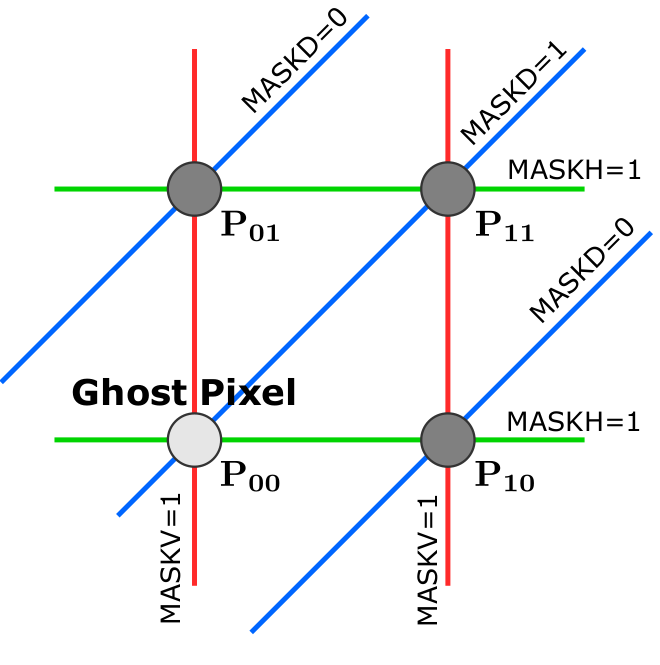
\includegraphics[width=.3\linewidth]{figures/Monopix1/masking_scheme.png}
        \caption{}
        \label{fig:masking_scheme}
    \end{figure}
    Un modo standard che si usa di solito è allocare un registro su ogni pixel periphery: il vantaggio di questo modo è che si può disabilitare ogni pixel individually. Questo metodo pur essendo più comodo richieda less amount of area ha però come drawback che il registro può essere soggetto a SEU \footnote{SEU = Single Event Upset, in sostanza è quando un bit ti cambia valore (da 0 a 1 o viceversa) perché una particella deposita carica nell'elettronica che fa da memoria (registro/RAM/...). Questo tipo di elettronica ha bisogno di un sacco di carica prima che il bit si "flippi" (cambi valore), infatti tipicamente per avere un SEU non basta una MIP che attraversa esattemente quel pezzo di chip in cui è implementata la memoria, ma un adrone che faccia interazione nucleare producendo più carica di quanto farebbe una MIP.} problema non trascurabile in acceleratori come HL-LHC adronici (TROVA UN ARTICOLO DOVE SI PARLA DI SEU).\\
    The implemented approch of masking in Monopix-1 funziona però solo se il numero di pixel da mascherare non è troppo alto dato che il numero di pixel unintentionally masked ("ghost pixels") increase with the number of pixels masked. \\
    Nel caso in cui solo due cordinate vengono utilizzate il numero di pixel unintentionally masked scales with $N^2$, where N is the number of the intentionally masked; if instead three coordinates are given the ghost pixels are $N^\alpha$ where $\alpha \min$2.\\

    R resistenza di reset deve essere abbastanza grande in modo da far si che il
    ritorno allo zero è abbastanza lento (non devi "interferire" con la tot slope
    e non devi più corto del tempo del preamplificatore, sennò hai perdita di segnale).\\
    Baseline reset: all'input solitamente hai un PMOSS o un diodo;  
    Voltage amplifier: perchè? ripeti un attimo il vantaggio. \\
    Source follower per disaccoppiare shaper e LF feedback.\\

    \subsection{FE parameters}
    Descrivo un po' le misure fatte sul fe e sul significato dei vari parametri.\\
    \begin{table}
        \begin{center}
        \begin{tabular}{|c | c |}
        \hline
        Parameter & Meaning\\
        \hline
        \hline
    
        \hline
        \end{tabular}
        \caption{}
        \label{tab:FE-parameters}
        \end{center}
     \end{table}
    
\section{Readout logic and Data-packets structure}
    TJ monopix ha un colum drain readout proven by the ATLAS FEI3 front end chip (
    I. Peric et al., The FEI3 readout chip for the ATLAS pixel detector,
    Nucl. Instrum. Meth. A 565 (2006) 178, ed. by J. Grosse-Knetter, H. Krueger, and N. Wermes
    (cit. on pp. 42, 50, 60))\\

    TJ-Monopix is a triggerless. It sends data whenever it gets hits. Only thing we can do is to record timetamp of the external triggers and correlate with the hits. 
    \begin{figure}[h!]
        \centering
        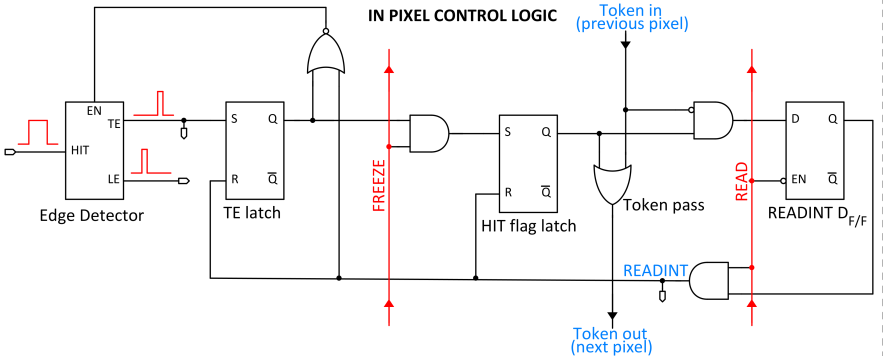
\includegraphics[width=.7\linewidth]{figures/Monopix1/Monopix1_readout_schematics.png}
        \caption{}
        \label{fig:Monopix1_readout_schematics}
    \end{figure}

    La lettura si può descrivere come una macchiana a stati in cui 

    
    \subsection{Dead time measurement}


\section{Applicability to FLASH}
Epitaxial layer thickness: più grande è e più carica viene depositata da una MIP, però devi fare attenzione alla forma della zona svuotata perchè può portare ad un aumento della charge sharing tra pixel vicini. Se il diodo è molto piccolo rischi che l'efficienza di collection è diminutia perchè l'intensità del campo elettrico è più bassa intorno al diodo, e hai più charge sharing.\\